%%%% Proceedings format for most of ACM conferences (with the exceptions listed below) and all ICPS volumes.
\documentclass[sigconf]{acmart}
%%%% As of March 2017, [siggraph] is no longer used. Please use sigconf (above) for SIGGRAPH conferences.

%%%% Proceedings format for SIGPLAN conferences
% \documentclass[sigplan, anonymous, review]{acmart}

%%%% Proceedings format for SIGCHI conferences
% \documentclass[sigchi, review]{acmart}

%%%% To use the SIGCHI extended abstract template, please visit
% https://www.overleaf.com/read/zzzfqvkmrfzn

\usepackage{booktabs} % For formal tables

% Copyright
%\setcopyright{none}
%\setcopyright{acmcopyright}
%\setcopyright{acmlicensed}
\setcopyright{rightsretained}
%\setcopyright{usgov}
%\setcopyright{usgovmixed}
%\setcopyright{cagov}
%\setcopyright{cagovmixed}


% DOI
\acmDOI{10.475/123_4}

% ISBN
\acmISBN{123-4567-24-567/08/06}

%Conference
\acmConference[WUWNet'17]{12th ACM International Conference on Underwater Networks and Systems}{November 2017}
{Halifax,NS,Canada}
\acmYear{2017}
\copyrightyear{2017}

\acmPrice{15.00}


\begin{document}
\title{
Matched-field source localization using sparsely-coded \\machine learning and data-model mixed training
%Neural Networks Based single-array passive source localization in shallow water
%Sparse Neural Networks Based Source localization for Underwater Networks % Array
%Neural Networks Based sensor-array data Sparse coding for Source Localization
%Data Based Sparse Learning for Underwater Sensor Array Networks
%:comparing with traditional matching field processing and a simpl15551621555162155516215551621555162e try of mixed data training
}
%Representation
\author{Shougui Cai}
\orcid{1234-5678-9012}
\affiliation{%
  \institution{College of Information Science and Electronic Eng. \\Zhejiang University}
  \streetaddress{}
  \city{Hangzhou}
  \state{China}
  \postcode{43017-6221}
}
\email{shouguicai@zju.edu.cn}

\author{Wen Xu}
\orcid{1234-5678-9012}
\affiliation{%
  \institution{College of Information Science and Electronic Eng. \\Zhejiang University}
  \streetaddress{}
  \city{Hangzhou}
  \state{China}
  \postcode{43017-6221}
}
\email{wxu@zju.edu.cn}

% The default list of authors is too long for headers}
\renewcommand{\shortauthors}{Shougui Cai.}


\begin{abstract}
%Developing methods to effectively clean and reduce the amount of data at sensor level is very meaningful for conveniently sharing and transferring information in underwater networks, due to the limitation of bandwidth and power supply.
Source localization is a basic task in ocean acoustics. The popularly used matched-field processing performs well only when the ocean environment is accurately modeled, due to its sensitivity to
the mismatch problem. In this paper, we view source localization as a machine learning problem and get a localization
prediction model by training a sparsely-coded feed-forward neural network.
Results on SWellEx96 experiment show that the learned model can achieve a good positioning performance in
source range estimation and has more ability to resist sound speed profile mismatch when trained by mixed environment model data,
compared with Bartlett processer. Machine learning based methods have a good potential for underwater source localization.
\end{abstract}

%
% The code below should be generated by the tool at
% http://dl.acm.org/ccs.cfm
% Please copy and paste the code instead of the example below.
%
\begin{CCSXML}
<ccs2012>
 <concept>
  <concept_id>10010520.10010553.10010562</concept_id>
  <concept_desc>Computer systems organization~Embedded systems</concept_desc>
  <concept_significance>500</concept_significance>
 </concept>
 <concept>
  <concept_id>10010520.10010575.10010755</concept_id>
  <concept_desc>Computer systems organization~Redundancy</concept_desc>
  <concept_significance>300</concept_significance>
 </concept>
 <concept>
  <concept_id>10010520.10010553.10010554</concept_id>
  <concept_desc>Computer systems organization~Robotics</concept_desc>
  <concept_significance>100</concept_significance>
 </concept>
 <concept>
  <concept_id>10003033.10003083.10003095</concept_id>
  <concept_desc>Networks~Network reliability</concept_desc>
  <concept_significance>100</concept_significance>
 </concept>
</ccs2012>
\end{CCSXML}

\ccsdesc[500]{Computer systems organization~Embedded systems}
\ccsdesc[300]{Computer systems organization~Redundancy}
\ccsdesc{Computer systems organization~Robotics}
\ccsdesc[100]{Networks~Network reliability}

% We no longer use \terms command
%\terms{Theory}

\keywords{Machine learning,%sparse coding,
source localization}

%\acmBadgeR{artifacts_available}

%% Used in some conference proceedings e.g. sigplan and sigchi
% \begin{teaserfigure}
%   \includegraphics[width=\textwidth]{sampleteaser}
%   \caption{This is a teaser}
%   \label{fig:teaser}
% \end{teaserfigure}

\maketitle

\section{Introduction}
As the increasing number of manned platforms deploying receiver arrays or  fixed/mobiled nodes in distributed underwater sensor networks,we are facing the scene of underwater big data.Due to the limitation of energy used,it is not realistically to process all the incoming data\cite{Yang2015Issues}.Now,machine learning technology is more and more mature, we could try to introduce some smart into our system,to extract task-relevent information,discover new patterns,construct a useful representation.It is convenient for us to share and transfer information between different platforms once the data can be reduced to small useful finite sets.

\section{Machine Learning Based Data Sparse Representation}
In Underwater Networks,we will get a lot of data. What we really care about,is not the signal itself,but the information contained in the siganl.Meanwhile,the communication for underwater sensors is costly.So develop methods to represent the information present in metadata with a sparse format is very meaningful.

In this section,we discuss an effective scheme using machine learning based methods.

\subsection{Neural Networks Models and Function Approximation}
As we known,neural networks models can be viewed as a mathematical function $f$.Taking feedforward neural network(FNN) as an example,they define a mapping ${\rm{y}}=f(x;\theta )$ between input $x$ and output $y$ by parameter $\theta$,which needed to be learned by a rule.Feedforward networks are called networks because they are typically represented by composing together many different functions.We might have two function $f^{1}$, $f^{2}$ connected in a chain\cite{goodfellow2016deep}, to form
$f(x) = f^{2}(f^{1}(x))$.

FNN extend linear models to represent nonlinear transformed format $\phi(x)$ of input $x$.The transform function $\phi$ can be thinked as providing a set of features describing $x$, or as providing a new representation for x.The key problem here is how to choose the mapping $\phi$.

The strategy of machine learning is to learn $\phi$.In a feedforward network,$\phi$ defines a hidden layer $h=\phi(x;w^{(1)})$,then the total model is $y=f(x;\theta,w)=hw^{(2)}$.
obviously,We need to learn $\phi$ from a broad class of functions,and parameters $w$ mapping $\phi(x)$ to the desired output.

In most cases,our parametric model defines a distribution $p(y|x;\theta)$.Simply, we can use the principle of maximum likelihood to learn parameters in model.
\begin{equation}
J(\theta ) =  - {E_{x,y \sim {p_{data}}}}\log {p_{\bmod el}}(y|x)
\end{equation}
where the specific form of $p_{\bmod el}$ is defined by networks.
As maximum likelihood is a consistent estimator, the model is capable of representing the training distribution.

\subsection{Regularization for neural networks}

There are two main kind of regularization strategys for neural networks,one is weight-level regularization,another is neuron-level regularization with activation penalty.
\begin{equation}
\tilde J(\theta ;X,y) = J(\theta ;X,y) + \alpha \Omega (\theta )+ \beta \Omega (h)
\end{equation}
where $\Omega (\theta )$ is parameter norm penalty, $\Omega (h)$ is penalty on the activations of the units,$\alpha$,$\beta$ are hyperparameters that weight the relative contribution of
the norm penalty term.Weight decay term penalize the size of the model parameters,while,the activation penalty term encouraging their activations to be sparse.

\subsection{Learn useful sparse representations from data}
When a useful sparse representation of any given data is learned,each datum will then be encoded as a sparse code,thus we can use the least possible amount of resource to store or transfer the data.
\begin{equation}
\begin{split}
&\tilde J(\theta ){\kern 1pt} {\kern 1pt} {\kern 1pt} {\rm{ = }}{\kern 1pt} {\kern 1pt} {\kern 1pt}  - {E_{x,y \sim {p_{data}}}}\log {p_{\bmod el}}(y|x){\rm{ + }}{\kern 1pt} {\kern 1pt} \lambda {\left\| h \right\|_1}\\
& s.t.{\kern 1pt} {\kern 1pt} {\kern 1pt} {\kern 1pt} {\kern 1pt} {\kern 1pt} {\kern 1pt} {\kern 1pt} {\kern 1pt} {\kern 1pt} {\left\| {{W_i}^{(1)}} \right\|_2} \le C{\kern 1pt} {\kern 1pt} {\kern 1pt} {\kern 1pt} {\kern 1pt} {\kern 1pt} {\kern 1pt} {\kern 1pt} {\kern 1pt} \forall {\kern 1pt} i = 1, \cdots ,M\\
\end{split}
\end{equation}
In practical application, we not only want the representation to be sparse,but also want the model features to be sparse, the latter saves the storage and calculation on sensor nodes. Thus,we use $L1$ norm to promote sparse neurons activations, and constrain the norm of each column of the weight matrix to prevent any one hidden unit from having very large weights. In the equation, $M$ is the number of neurons in hidden layer.

\section{Simulation and experimental results}
A notable recent example of using machine learning method in underwater acoustic is the application of nonlinear classification to source localization\cite{niu2017source}.
In this section,we implement a simple FNN with just one hidden layer to learn source range directly from observed acoustic data,
and compare the performance of the classifier with the traditional matching field processing method (Bartlett) in terms of simulation data and experimental data, respectively.In addition, we briefly discuss the influence of sound speed profile(ssp) mismatch on the performance of FNN classifier and improve the tolerance of the classifier by training the model using data sampled under different ssp.

Simulation environment is the widely studied SWell96Ex test,conducting in a 216m deep shallow waveguide environment.The ship proceeded northward at a speed of 2.5 m/s.

The source ship has two sound source, a deep source (J-15) and a shallow source (J-13).In all the simulations, we used the shallow sound source,
which was towed at a depth of about 9m and transmitted 9 frequencies between 109Hz and 385Hz.

\subsection{Parameter Settings}
In simulation part,acoustic data used to train and test the neural network is generated by kraken.Snapshot $N_{s}$ is 10,number of vertical array elements $L$ is 21,input layer neurons $D$ of FNN is $L^{2} \times N_{fre}$(number of frequency used),there is an input data preprocessing here, actual input data is the normalized sample covariance matrices(CSDM) of measured pressure at each frequency. The number of neurons in the output layer (number of classes) $K = 300$.We just give the same amount of dimensions the original data are encoded in to provide enough dimensions to learn over-complete features at first,which means neurons in hidden layer $M = D$. Specifically,the cost function now becomes
\begin{equation}
\begin{split}
&\min {\kern 1pt} {\kern 1pt} {\kern 1pt} {\kern 1pt} {\kern 1pt} {\kern 1pt} \tilde J(\theta ){\kern 1pt} {\kern 1pt} {\kern 1pt} {\rm{ = }}{\kern 1pt} {\kern 1pt} {\kern 1pt} {\rm{ - }}{{\rm{1}} \over N}\sum\limits_{n = 1}^N {\sum\limits_{k = 1}^K {{t_{nk}}\ln {y_{nk}}{\kern 1pt} {\kern 1pt} {\kern 1pt} {\rm{ + }}{\kern 1pt} {\kern 1pt} \lambda {{\left\| h \right\|}_1}} }\\
& s.t.{\kern 1pt} {\kern 1pt} {\kern 1pt} {\kern 1pt} {\kern 1pt} {\kern 1pt} {\kern 1pt} {\kern 1pt} {\kern 1pt} {\kern 1pt} {\left\| {{W_i}^{(1)}} \right\|_2} \le C{\kern 1pt} {\kern 1pt} {\kern 1pt} {\kern 1pt} {\kern 1pt} {\kern 1pt} {\kern 1pt} {\kern 1pt} {\kern 1pt} \forall {\kern 1pt} i = 1, \cdots ,M\\
\end{split}
\end{equation}
where $t_{nk}$ and $y_{nk}$ are predictive and real probability of sample data $x$ belongs to class $k$ separately.Moreover we will choose $C=1$ here.
For the sake of learning speed ,we use the $ReLU$ activation in hidden layer and use the $softmax$
function in the output layer because this case is a multiple class problem.
The training set is 3000 samples of uniform sampling between 1.82\--8.65km,test set is another 300 data samples sampling from the same range.The noise in the simulation is set to complex gaussian white noise.

Experimental data gets from SWell96Ex Event S5,we use the receive sound pressure of VLA to train our neural network.The array recorded a total of 75 min of data,In order to facilitate processing, we took 0\--50min data as a training set.

Consistent with the simulation part,we divide the trajectory into 300 grids,25m each.We set 1 second as a snapshot and get 3000 sample covariance matrix (SCM),the sample covariance matrix is averaged at every two snapshots.
At the time of training, we took 9/10(2700)of samples as training set and another 1/10(300) as test set.

\subsection{The Effect of Sparse Constraint Training}
The regularization degree on model affects the model error and average activation density of FNN's hidden layer. As the coefficient grows, the model error on training set and test set also grows, but slower on test set, which means 
the regularization helps improving the performance on test data in some sense. The model error is defined as the dissimilarity between true probability distribution and estimated probability distribution, thus the Kullback-Leibler(KL) divergence. 
In Fig.2, we use the cross entropy equivalently.

On the other hand, the regularization on neuron-level significantly reduces the average activation density, 
The order of magnitude drops from $10^{3}$ to $10$, and keep it stably. This phenomenon is a good news for 
us to train a sparse representation form data. 

Compared to the case of training without sparse constraints, sparse constraint makes the weight coefficient in the hidden layer show the group structure,either all zero, or basic is not zero. Take the case $\lambda=3.5 \times 10^{-5} $ 
for example, the number of feature vectors reduced from 1500 to 140, as shown in Fig.1. In addition, it can be seen that the relative size of learned weights is related to the frequency,even at the same frequency, the the weight corresponding 
to real and imaginary parts is also different, there are bright and dark strip distribute along the data dimension.The data dimension is arranged according to the frequency relationship.

\begin{figure}
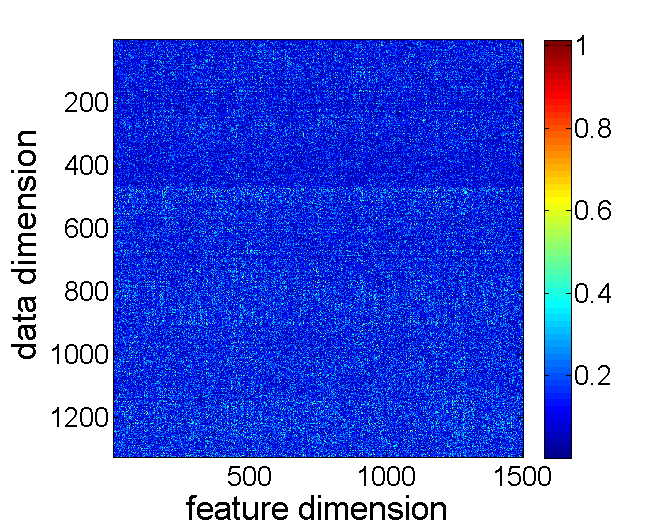
\includegraphics[width=4cm,height=3cm]{figure/Weights_summaries_in_hidden_laye_swell_exp}
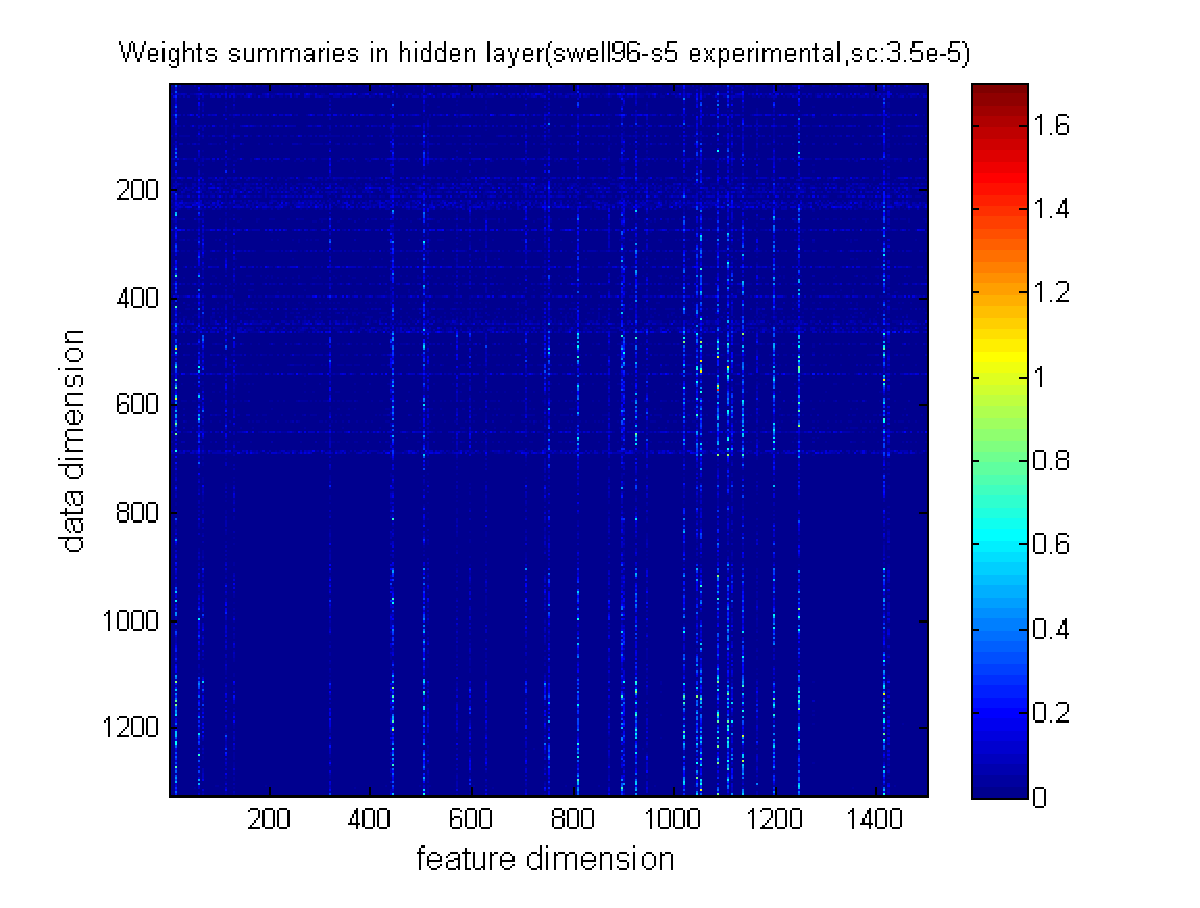
\includegraphics[width=4cm,height=3cm]{figure/Weights_summaries_in_hidden_laye_swell_exp_sc_3dot5_e_neg_5}
\caption{weights summaries in hidden layer(left:no constraint,right:with constraint).}
\end{figure}

\begin{figure}
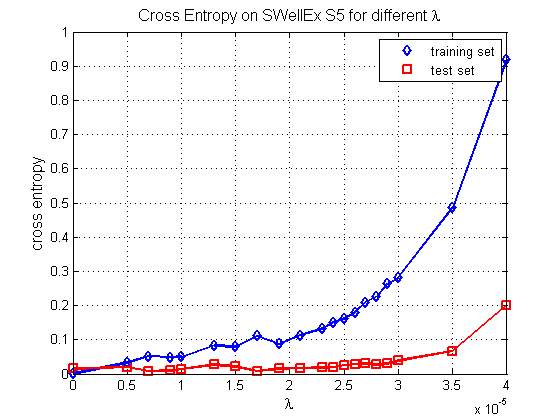
\includegraphics[width=4cm,height=3cm]{figure/Cross_Entropy_on_SWellEx_S5_for_different_lambda}
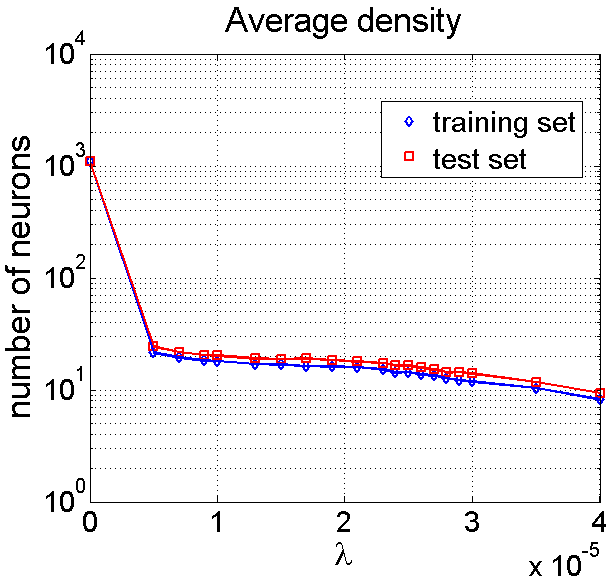
\includegraphics[width=4cm,height=3cm]{figure/Hidden_Average_Density_on_SWellEx_S5_for_different_lambda}
\caption{Model error and Average-activation-density for different $\lambda $.}
\end{figure}


%\begin{figure}
%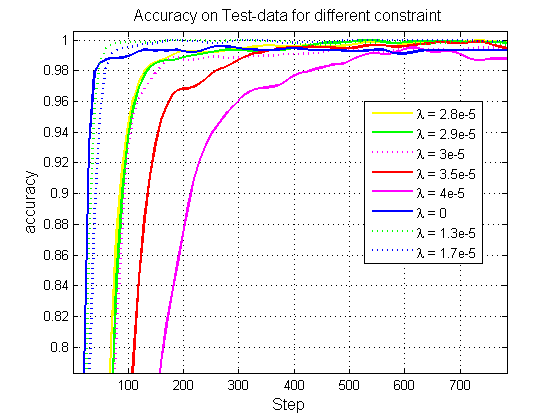
\includegraphics[width=4cm,height=3cm]{figure/Accuracy_on_Test_data_for_different_constraint_exp}
%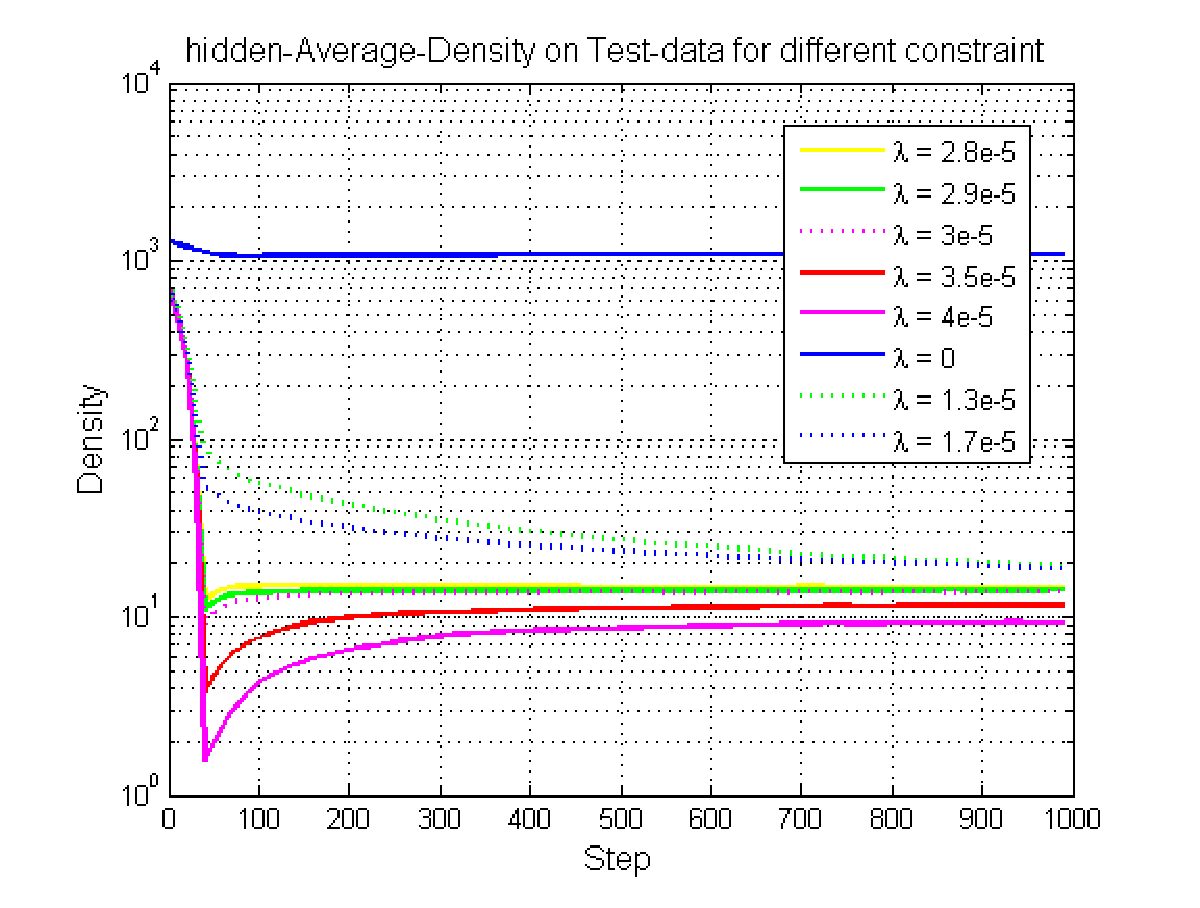
\includegraphics[width=4cm,height=3cm]{figure/hidden-Average-Density-on-Test-data-for-different-constraint_exp}
%\caption{Accuracy and Average-Density on test data for different-constraint.}
%\end{figure}

%\begin{figure}
%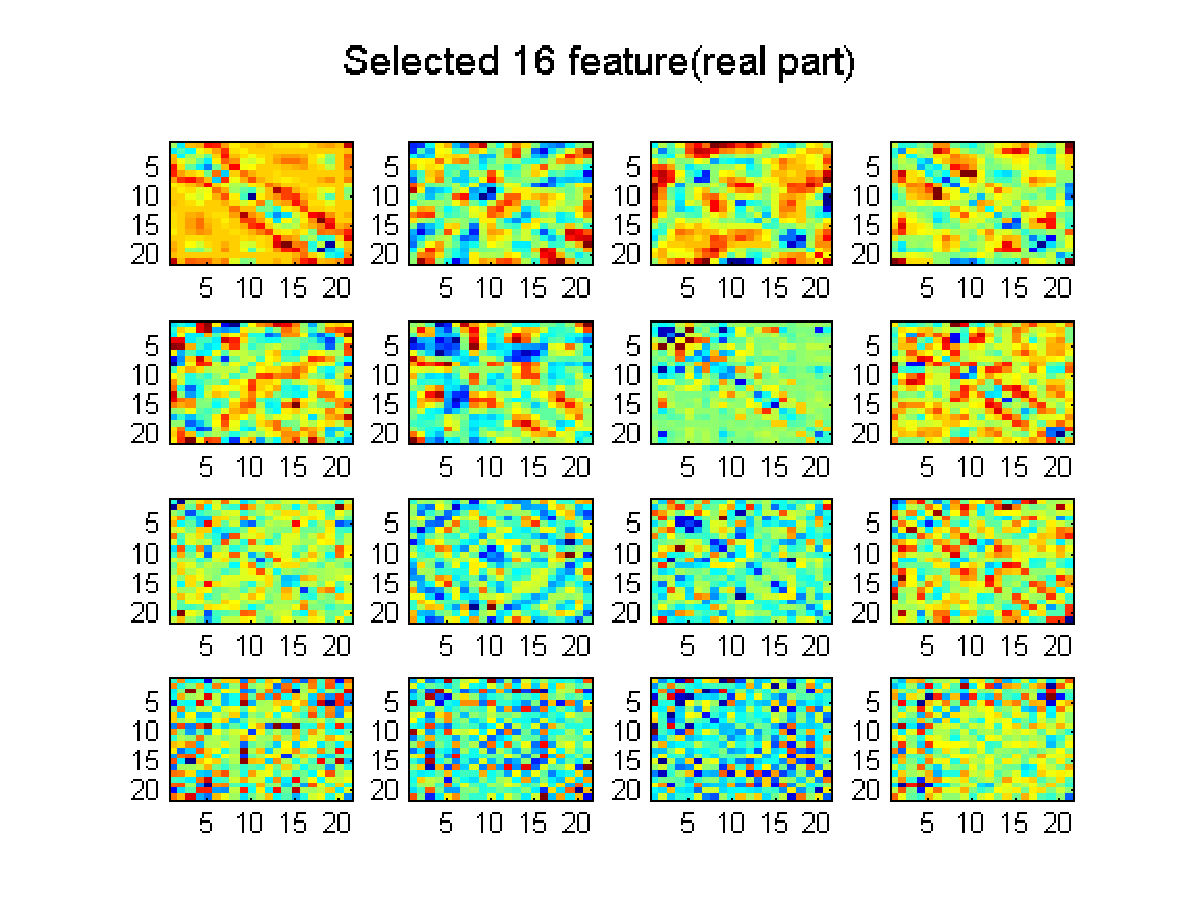
\includegraphics[width=4cm,height=3cm]{figure/selected_16_features_real_part}
%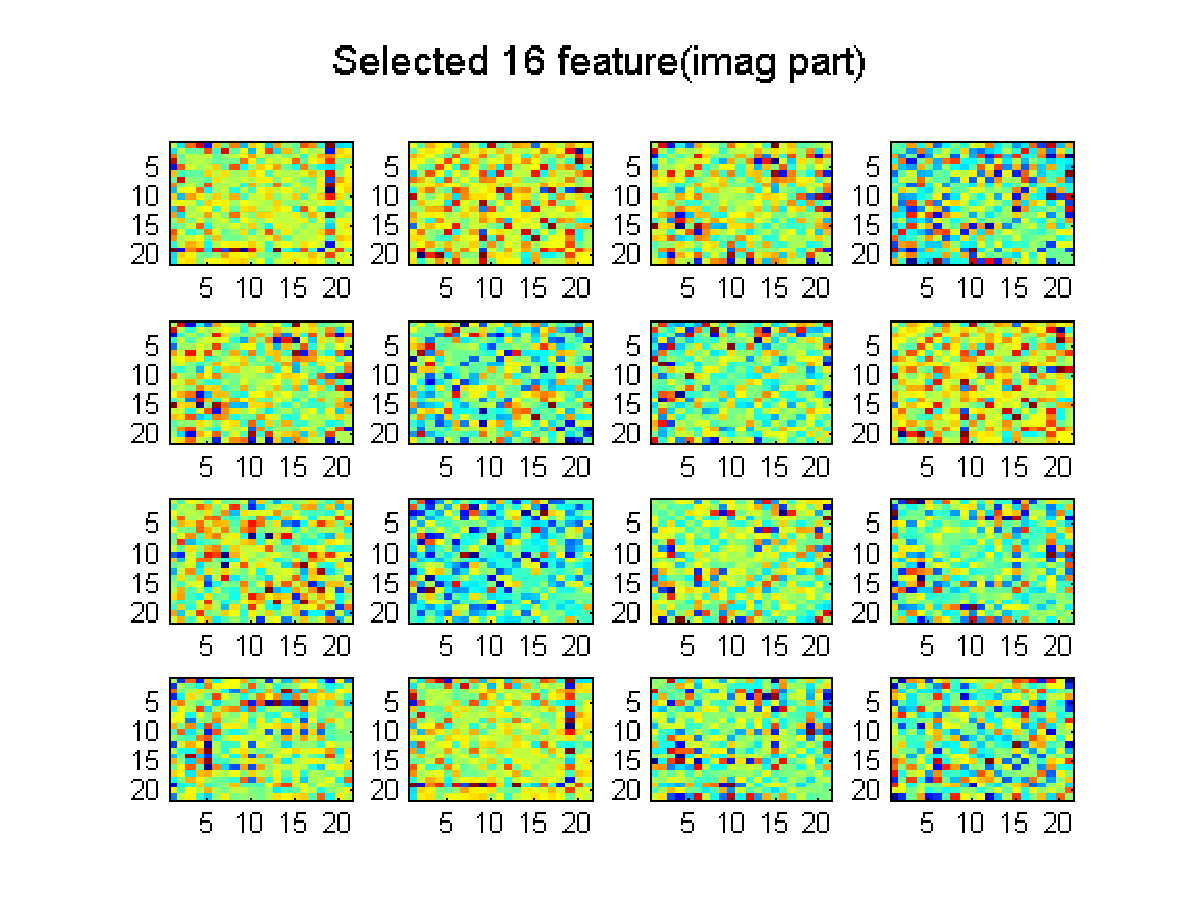
\includegraphics[width=4cm,height=3cm]{figure/selected_16_features_imag_part}
%\caption{Selected 16 features learned by neural network.}
%\end{figure}

\begin{figure}
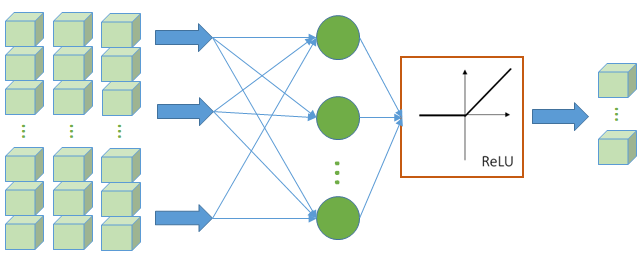
\includegraphics[width=8cm]{figure/sparse_represention_model}
\caption{The learned sparse representation model.}
\end{figure}

Apart from being beneficial to feature selection,sparse constraint can reduce the activation rate of neurons in the hidden layer, without significant reduction in accuracy. In our example, when the coefficient is 3.5e-5, the average activation neuron number is 11,which is greatly reduced,the activation rate is only 0.7{\%}.
These mean the input 1323-dimension data can be represented by only 140 feature vectors.Evean more, averagely, each data sample can be represented by only 11 feature, as Fig.1 showns.The metadata is being compressed well. To sum up, by using regularization strategy on neural networks, we get a sparse and low rank model, where sparse means the transferred representation is sparse, low rank means the rank of learned weight matrix is low. The learned sparse representation model is Illustrated in Fig.3. 
A sparse vector can be formed by filtering the data measured in sensor nodes through the pretrained neuron networks. Decisions, such as target location can be made by further processing.

\subsection{Comparison with traditional matching field processing method}
As a reference,here we use Bartlett Processor to position the source position.There are two kinds of replica-field used in Bartlett Processor,one is calculated from model by kraken(noted as bartlett 2), another is from measurement data(noted as bartlett 1), same as the training data used in FNN.
% Please add the following required packages to your document preamble:
% \usepackage{booktabs}
\begin{table}[]
\caption{Localization accuracy of FNN and MFP on SWell96Ex-S5 data}
\label{my-label}
\begin{tabular}{@{}lllll@{}}
\toprule
Methods       & FNN    & MCE    & Bartlett 1 & Bartlett 2 \\ \midrule
109Hz         & 89.3\% & 72.3\% & 37.7\%     & 3.7\%      \\
232Hz         & 97\%   & 91\%   & 17.7\%     & 4.3\%      \\
385Hz         & 99.7\% & 97.7\% & 14\%       & 0.67\%     \\
109,232,385Hz & 99\%   & 99.7\% & 40.7\%     & 7.7\%      \\ \bottomrule
\end{tabular}
\end{table}

% Please add the following required packages to your document preamble:
% \usepackage{booktabs}
\begin{table}[]
\caption{Absolute mean error of FNN and MFP on SWell96Ex-S5 data(m)}
\label{my-label}
\begin{tabular}{@{}lllll@{}}
\toprule
Methods       & FNN  & MCE   & Bartlett 1 & Bartlett 2 \\ \midrule
109Hz         & 28.1 & 290.3 & 852.8      & 1219.5     \\
232Hz         & 7.4  & 2.5   & 832.3      & 832.3      \\
385Hz         & 0.08 & 0.58  & 1266.7     & 1756.3     \\
109,232,385Hz & 0.25 & 0.083 & 477.2      & 722.9      \\ \bottomrule
\end{tabular}
\end{table}

The accuracy and absolute mean error of different methods under different frequency are summed in table 1 and table 2. As we can see, whether it is in single frequency or in combination frequency,the accuracy of FNN is always better than Bartlett, and not worse than direct data match(noted as MCE), whcih is more obvious when it come s to the comparison of absolute mean error. Thus, the study of neuron networks based sparse representation model is meaningful in positioning problem. 

\subsection{The influences of ssp mismatch on FNN classifier}
In the MFP method, the model accuracy is heavily affected by the mismatch problem. Fig.5 gives the FNN positioning results by simulatuons in different degrees change of sound speed profiles. Here, snapshot is 10 and snr is 5dB.
\begin{figure}
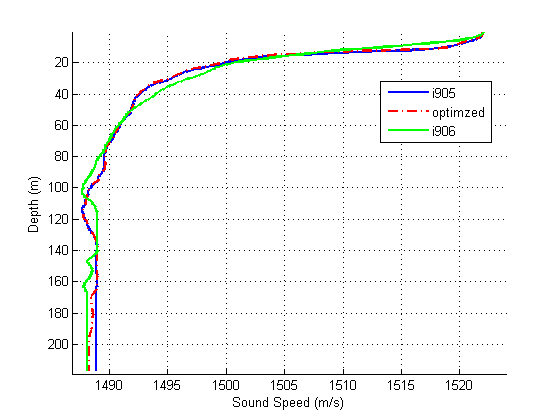
\includegraphics[width=6cm,height=5cm]{figure/ssp3}
\caption{plot of sound speed profiles.}
\end{figure}
Comparing to optimized-ssp,the i905-ssp has only a very small change,within 0.5m/s at the same depth.The change in i906-ssp is much significant,which can be seen from the shape in Fig.4.
\begin{figure}
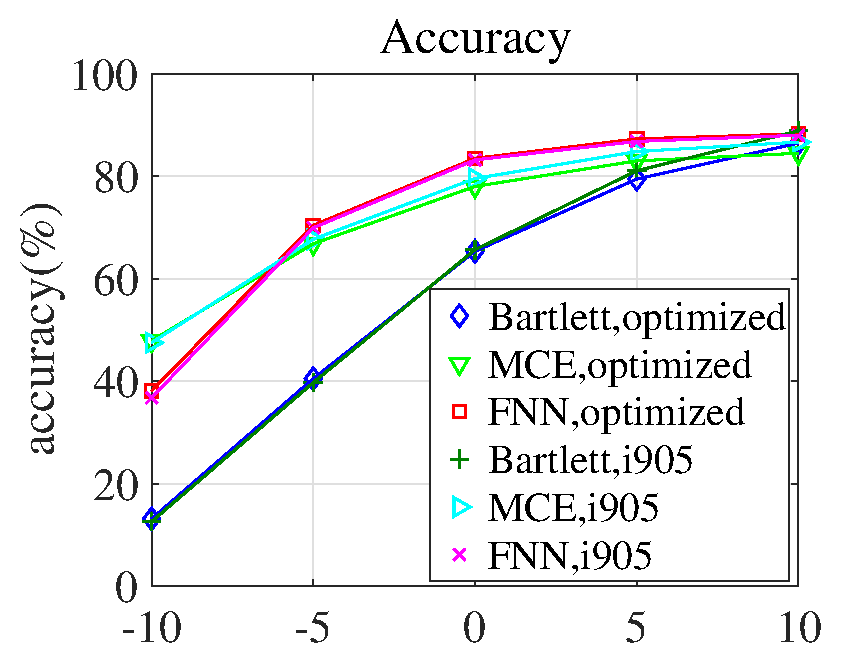
\includegraphics[width=4cm,height=3cm]{figure/Accuracy_to_SNR_FNN_vs_Bartlett_MCE}
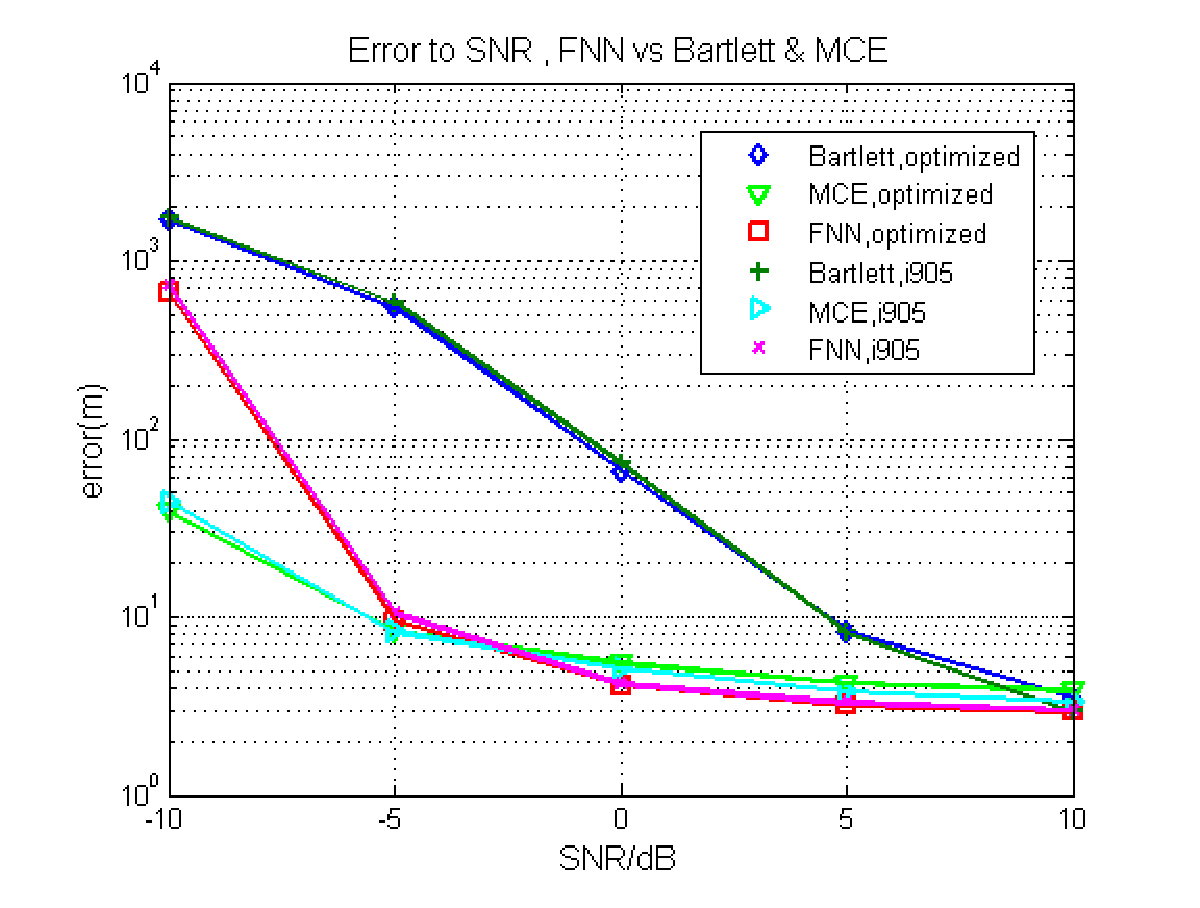
\includegraphics[width=4cm,height=3cm]{figure/Error_to_SNR_FNN_vs_Bartlett_MCE}
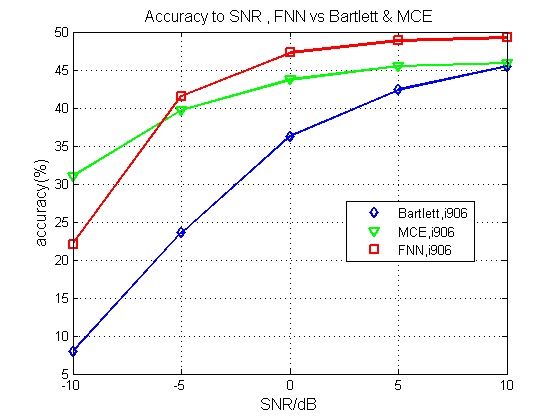
\includegraphics[width=4cm,height=3cm]{figure/Accuracy_to_SNR_FNN_vs_Bartlett_MCE_i906}
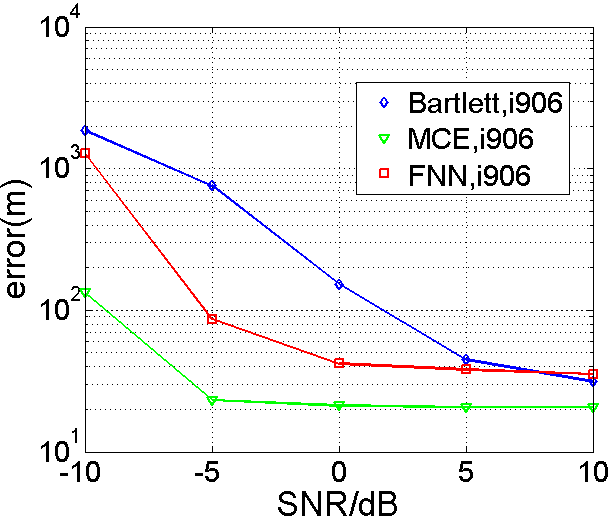
\includegraphics[width=4cm,height=3cm]{figure/Error_to_SNR_FNN_vs_Bartlett_MCE_i906}
\caption{FNN positioning performance curve on simulation data
(frequency:109,232,385Hz).}
\end{figure}

 The performance curves for FNN, Bartlett, MCE is ploted by 1000 times Monte Carlo simulation in Fig.5. When the change in ssp is relatively small(the up two sub figures), FNN positioning best, MCE second and Bartlett worst. 
 When the shape of ssp change(the down two figures), the accuracy order unchanged, but the absolute error of FNN becomes bigger than MCE.


\subsection{%Co-training using data collected from different ssp
Increase model tolerance by mixed data training}
The simulation results show that training the model using data collected from different ssp can significantly improve the tolerance of the classifier,which means FNN can learn weigths over a set of changing ssp.This is an interesting and useful discovery.

%\begin{figure}
%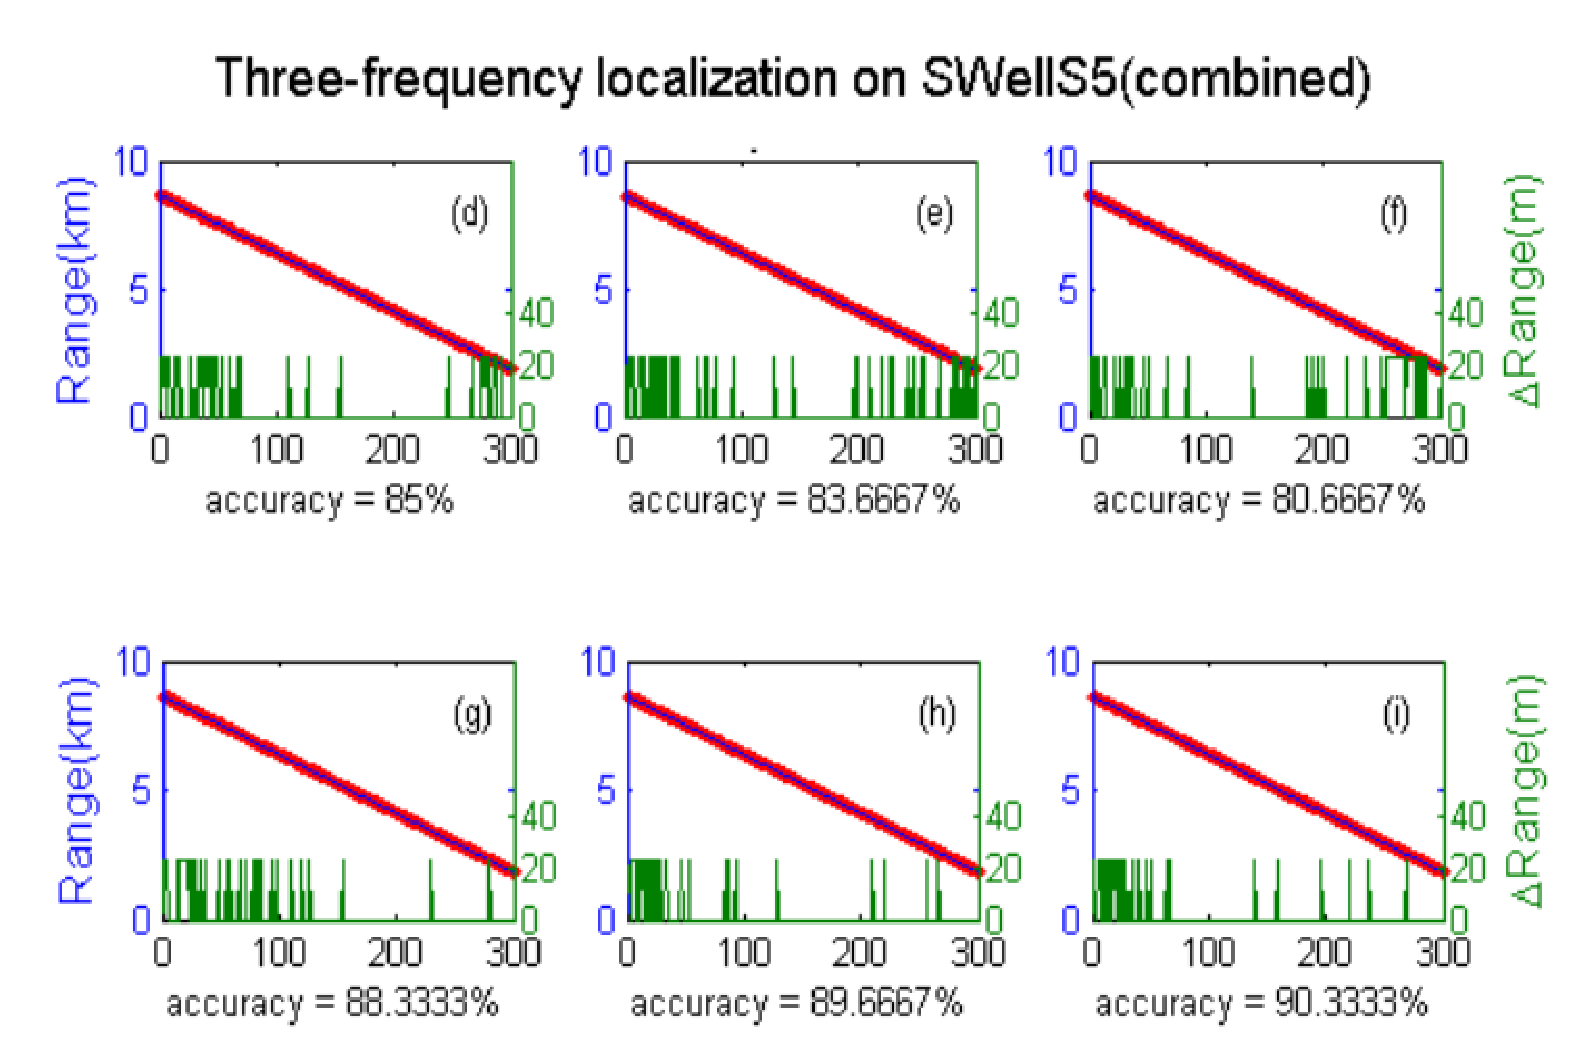
\includegraphics[width=4cm,height=3cm]{figure/combinevssingle_lef}
%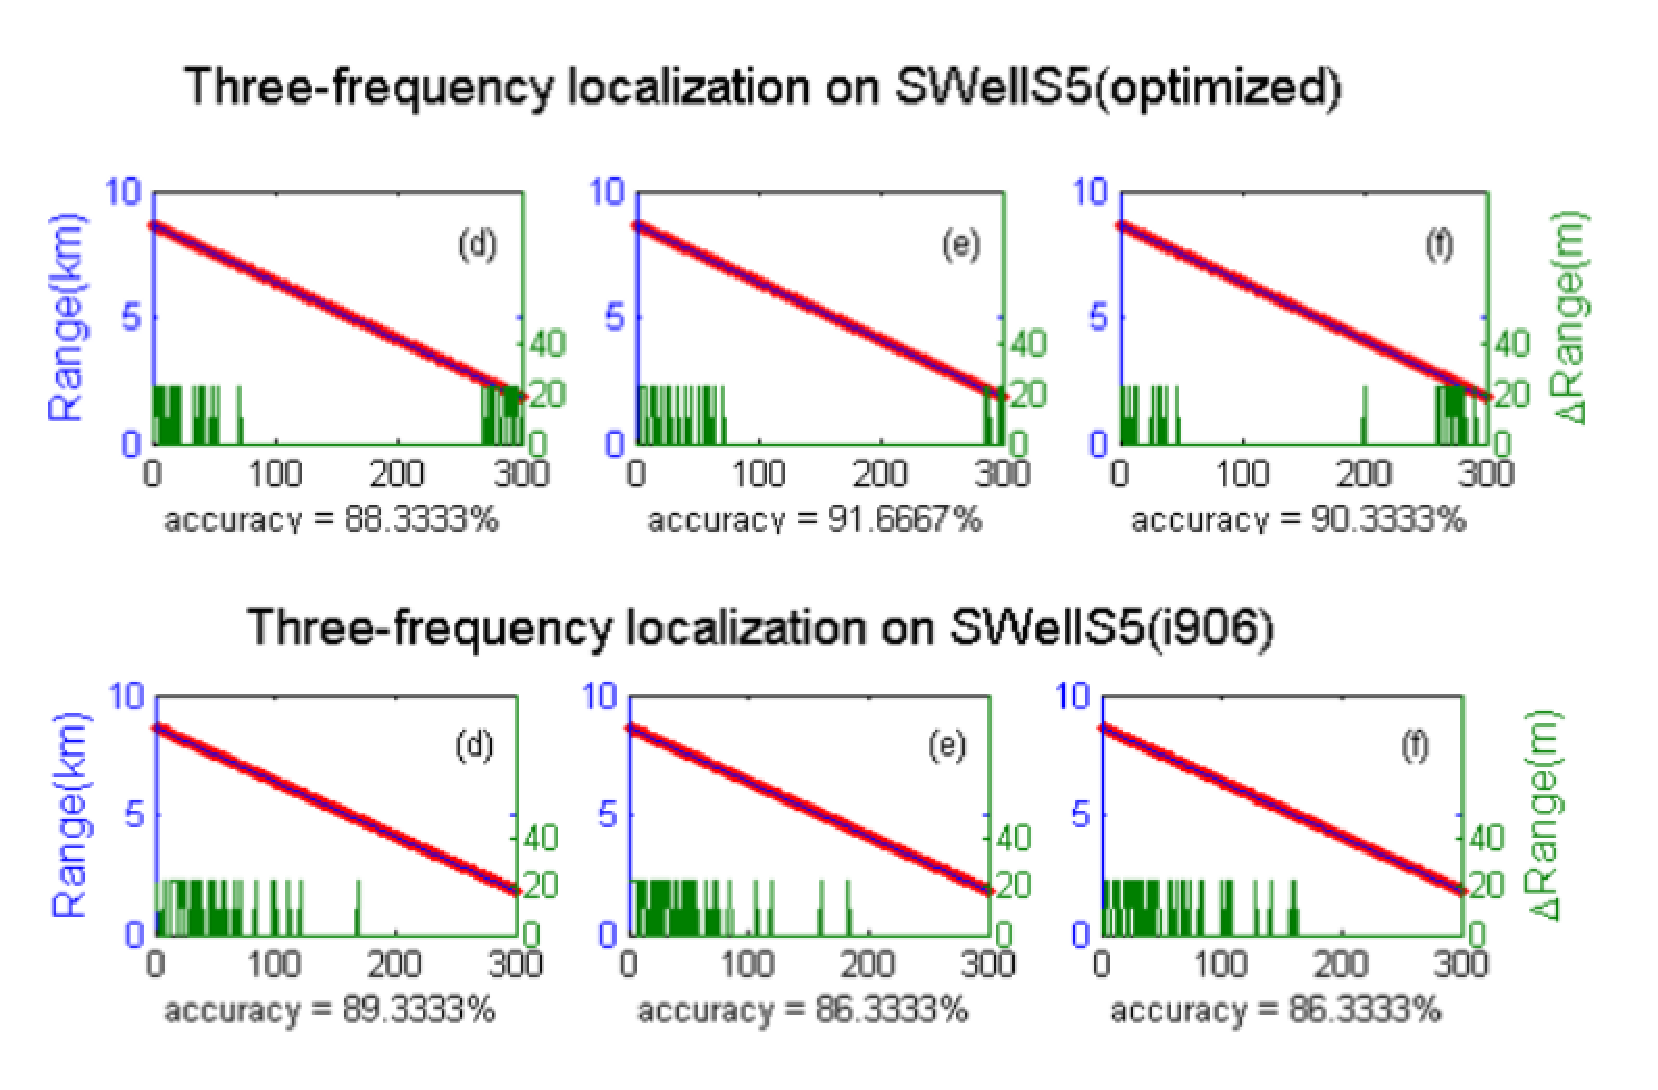
\includegraphics[width=4cm,height=3cm]{figure/combinevssingle_right}
%\caption{Comparison of mixed data training and single data training .}
%\end{figure}

As dicussed in section 3.4, the FNN is also sensitive to ssp mismatch, but still perform better than Bartlett. When the environment ssp has a big change in the shape(such as from ssp-optimized to i906), the performance of the estimator drops about 40\% in accuracy. In this section, by adding some data collected form i906-ssp, the positioning ability of FNN on i906{*}(which is little changed from i906,for the sake of testing) is as better as before. Although the accuracy for i905 has a little glissade compared with single data training, the performance for i906 imporved. In general, the trained FNN classifier works well on both two different shape ssp.Note that, the legend 'i905,combined' means the model is trained by mixed data collected from ssp i906 and ssp optiminized, then the model is tested on ssp i905, rests is similar.

\begin{figure}
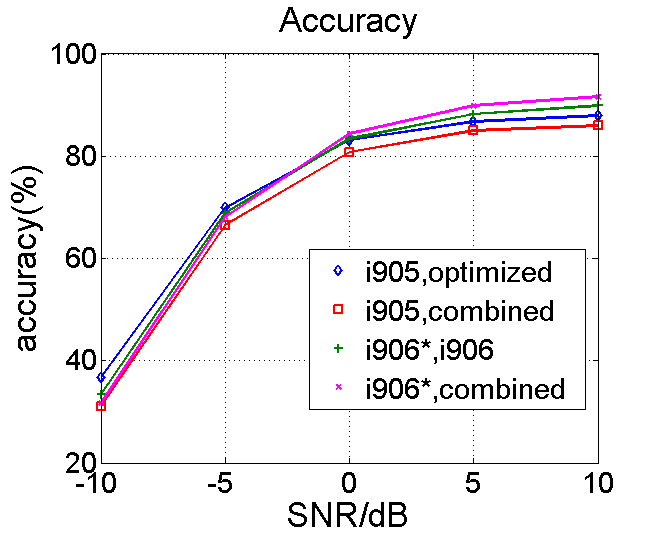
\includegraphics[width=4cm,height=3cm]{figure/Accuracy_to_SNR_Combined_vs_Single}
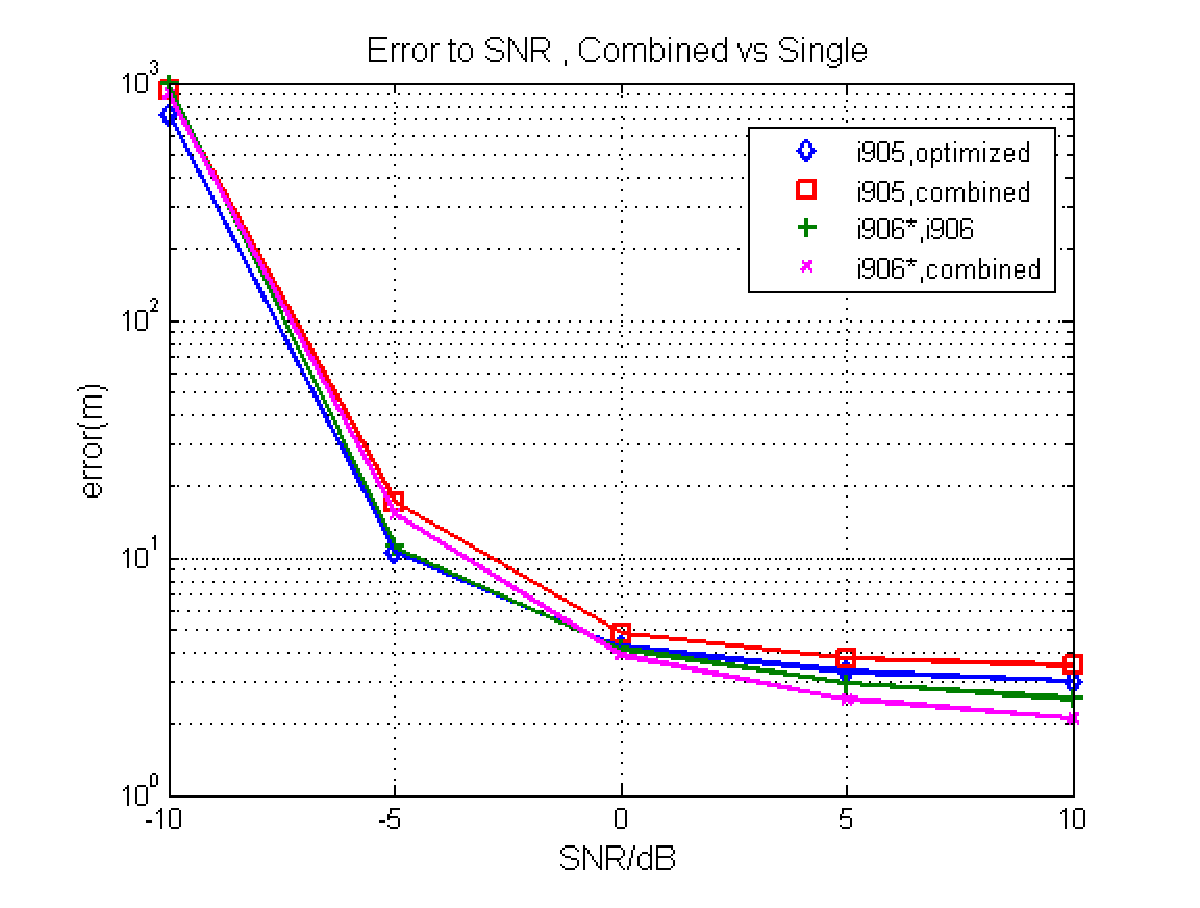
\includegraphics[width=4cm,height=3cm]{figure/Error_to_SNR_Combined_vs_Single}
\caption{FNN positioning performance curve on simulation data.}
\end{figure}

\section{Conclusions}
%In a recent article\cite{niu2017source}, Niu considers the problem of sound source location in marine waveguides as a classification problem under the framework of machine learning,and verified the ideal on the Noise09 experimental data.
From the veiw of information theory, the objective of signal processing is to exact specific task-relevant information from data.
How to exact the relevant information from measured data is an important issue.Machine learning may be able to provide ideas for this issue, because of its strong ability to learn and characterize.
In this paper,we develop a method to learn sparse representation from data based on neural networks.At present, we only discuss the situation of a single linear array, the situation for multi-array will be dicussed in future.
Verification on SWell96Ex experimental data shows this method can help select feature vectors and extract task-related information contained in the siganl. The pretained sparse repesentation model can help the underwater networks use the least possible amount of resource to store or transfer the data. Compared to the traditional MFP method, the neural network trained model have more ability to resist sound speed profile mismatch and can fine-tune to a feature extractor conveniently.

\begin{acks}
The work is supported by ...

\end{acks}


%\bibliographystyle{ACM-Reference-Format}
\bibliographystyle{unsrt}
%\bibliography{sample-bibliography}
\bibliography{acmart}

\end{document}
